\chapter{Experimentální uspořádání} \label{exp_usporadani}
Jediný vzorek, který byl v rámci této práce studován, je vzorek GaMnAs s~označením F002, který je popsán v kapitole \ref{kap_vzorek}.

Použili jsme laser Thorlabs LDM785 s vlnovou délkou $\lambda=\SI{785}{\nm}$.

Všechna měření jsme prováděli v jedné ze dvou geometrií. V nekolineární geometrii, ve které laserový svazek nedopadá přímo kolmo na vzorek a odražený svazek je tedy vychýlený a dobře oddělený od vstupujícího svazku, jsme provedli měření hysterezních smyček. Stejná měření na stejném vzorku byla již provedena v práci \cite{Reichlova}. Cílem tohoto měření bylo ověření funkčnosti setupu.

Poté jsme přešli do kolineární geometrie (kolmý dopad na vzorek). V ní je vzorek i magnetické pole v rovině kolmé na směr šíření svazku. V této geometrii jsme provedli všechna zbývající měření.


\subsubsection*{Soustava souřadná}
Osu $z$ ztotožňujeme s osou elektromagnetu a chodem paprsku před dopadem na vzorek. Laser tedy svítí ve směru vektoru $-\vec{z}$.
Osa $x$ míří dolů a osa $y$ při pohledu ve směru svazku doprava ($xyz$ tvoří pravotočivou soustavu). Viz obr. \ref{souradna_soustava_vzorek}.

Elektromagnet dokáže při tomto označení generovat magnetické pole $\vec{H}_{\text{ext}}$ v~rovině $xy$.

Všechny úhly v rovině $xy$ (vnější pole $\phH$, magnetizace $\phM$, rovina polarizace $\beta$, bisektrisa snadných os $\gamma$, úhel mezi snadnými osami $\xi$) měříme od osy $x$ směrem k ose $y$. $\vec{x}$ je tedy ve směru \ang{0} a  $\vec{y}$ ve směru \ang{90}.


Podle \cite{TesarovaDisertace} mají být snadné osy vzorku v našem uspořádání ve směrech \ang{59}, \ang{121}, \ang{239}, \ang{301} ($\pm$~\ang{5}). Bisektrisa dvou přilehlých snadných os je ve směru $\gamma=\ang{90}$.


\begin{figure}[htbp]\centering
	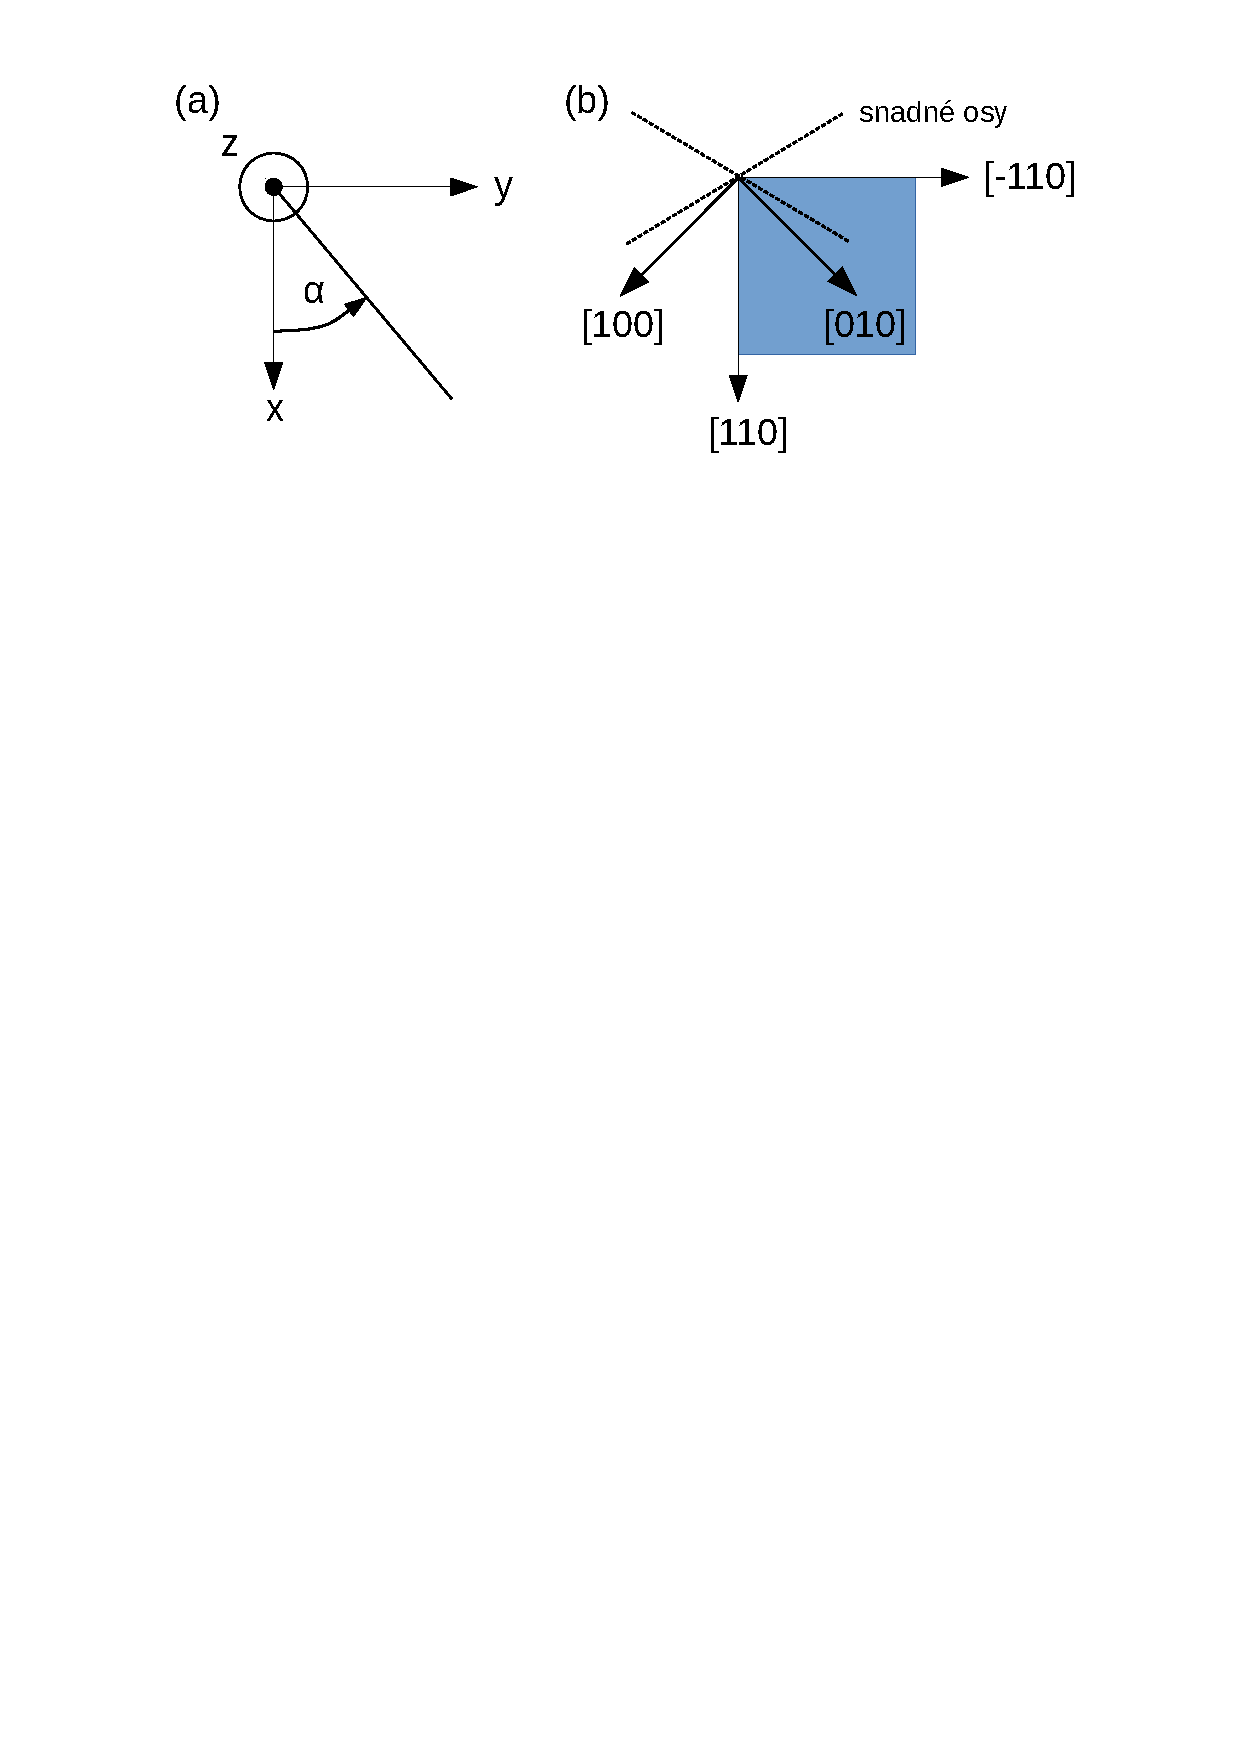
\includegraphics[trim={1in 8.5in 1in 0.5in}, clip, width=\textwidth]{./png/soustava}
	\caption{(a) Zavedení soustavy souřadné. Pohled ve směru chodu paprsku dopadajícího na vzorek. (b) Umístění vzorku na studeném prstu kryostatu.}\label{souradna_soustava_vzorek}
\end{figure}


\subsubsection*{Nekolineární geometrie}

Schéma experimentálního uspořádání v nekolineární geometrii je na obr. \ref{nekolinearni_usporadani}.

Po výstupu z laseru svazek nejprve prochází modulátorem intenzity (přerušovač svazku).
Svazek dále prochází dvěma polarizátory s osou ve směru \ang{0}, mezi kterými je umístěna $\lambda/2$ fázová destička kvůli nastavení intenzity vystupujícího světla. Vystupující polarizace je lineární $\beta=\ang{0}$.

Následuje $\lambda/2$ fázová destička, pomocí které nastavujeme rovinu polarizace $\beta$ světla dopadajícího na svazek. Svazek je dále fokusován \SI{5}{D} spojnou čočkou na vzorek, který je umístěn mezi pólovými nástavci magnetu. 

Vzorek mírně vykloněn z roviny $xy$, takže se odražený svazek odchyluje od dopadajícího. Úhel mezi dopadajícím a odraženým svazkem je $\ang{6,6}\pm\ang{0,5}$, úhel dopadu na vzorek je tedy $\ang{3,3}\pm\ang{0,3}$.
Odražený svazek koliminujeme další \SI{5}{D} spojnou čočkou.

Zbývající část uspořádání se označuje jako \emph{optický můstek}. Podrobný popis lze nalézt např. v \cite{Rozkotova}. Hlavní komponentou můstku je polarizátor, který svazek rozdělí na svislou a vodorovnou polarizaci. Před můstkem je umístěna vyvažovací $\lambda/2$ fázová destička s piezo ovládáním, pomocí které otáčíme rovinu polarizace tak, aby intenzita v obou ramenech byla stejná. Oba svazky dále fokusujeme do detektorů.
Detektory jsou připojené na dva elektronické směšovače, které signály z obou detektorů sečtou (A+B) a odečtou (A-B). Oba směšovače jsou připojené do fázově citlivých zesilovačů (\emph{lock-in}).
Hlavní výhodou optického můstku je, že měříme přímo rozdílový signál a vyhneme se tím odčítání blízkých čísel. Navíc fluktuace v intenzitě laseru se rovnoměrně rozdělí do obou ramen a odečtou se.

Z lock-inů dostáváme dva signály $I_{A+B}$ a $I_{A-B}$. Pokud při určitém polarizačním stavu světla vyvážíme můstek a následně dojde ke stočení roviny polarizace, dojde také k rozvážení můstku. Pro malé úhly ho můžeme určit jako \cite{Rozkotova}
\begin{equation} \label{e:mustek}
\beta = \pm\frac{I_{A-B}}{2I_{A+B}} \,,
\end{equation}
kde znaménko $+$, nebo $-$ závisí na tom, v jaké ze dvou vyvažujících poloh je vyvažovací $\lambda/2$ destička, a který z detektorů detekuje jakou polarizaci. My jsme znaménko určili z měření v kapitole \ref{kap_toceni}. Stejný jev měříme pomocí Voigtova jevu (z~rozdílového signálu) a MLD (ze součtového signálu). MLD nám dovoluje jednoduše určit znaménko jevu, a protože Voigtův jev by měl dát tu samou informaci, tak určíme správné znaménko.

Použité směšovače nejsou totožné a při stejném zesílení se jejich výstupní napětí liší až o \SI{5}{\percent}, ale korekci na tuto skutečnost neprovádíme.

\begin{figure}[htbp]\centering
	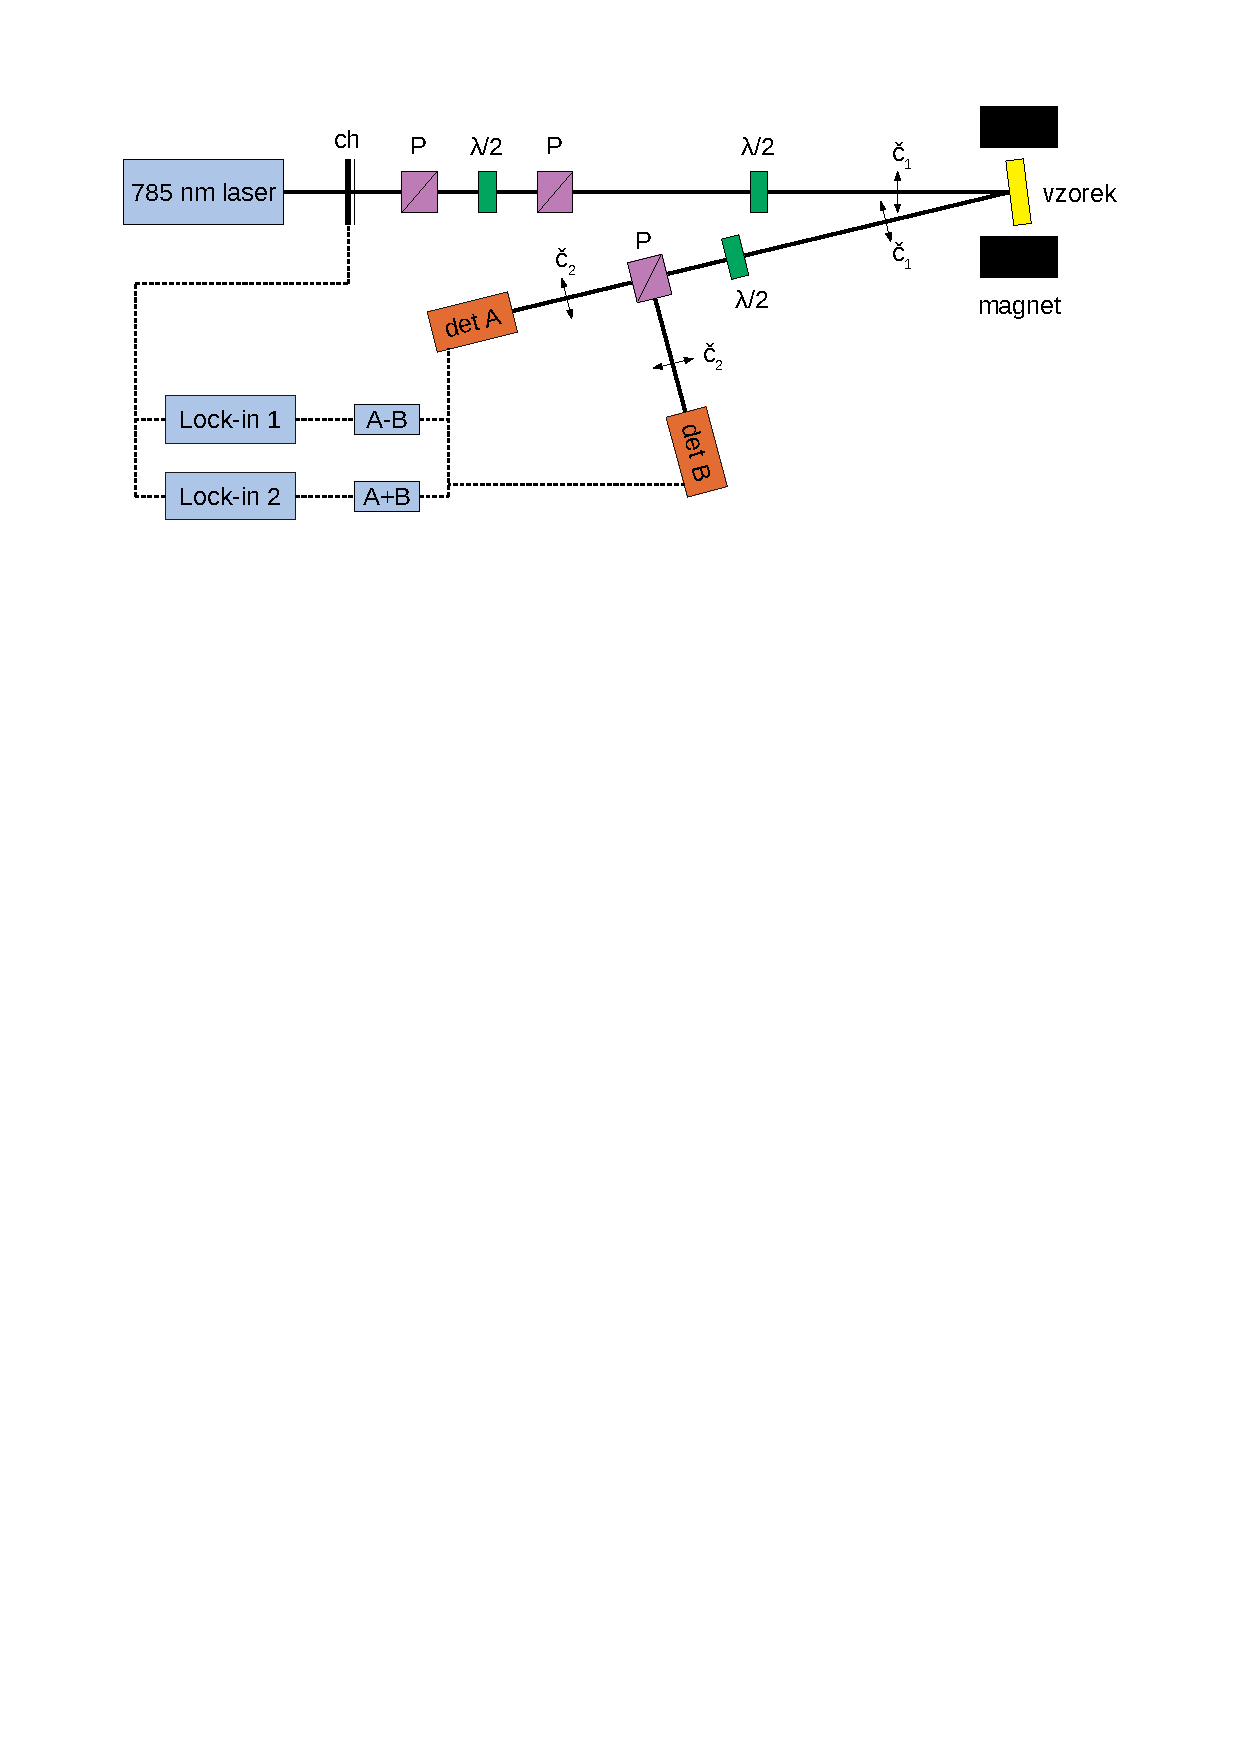
\includegraphics[trim={0,7in 8in 0,7in 0.5in}, clip, width=\textwidth]{./png/nekolinearni_usporadani}
	\caption{Experimentální uspořádání v nekolineární geometrii. ch --- přerušovač svazku, P --- polarizátor, $\lambda/2$ --- půlvlnná destička, č$_\text{i}$ --- spojná čočka.}\label{nekolinearni_usporadani}
\end{figure}

\FloatBarrier

\subsubsection*{Kolineární geometrie}
Schéma experimentálního uspořádání v kolineární geometrii je na obr. \ref{kolinearni_usporadani}.

První část uspořádání je stejná. Vzorek je však nyní kolmo na dopadající svazek a ten se tedy vrací stejnou drahou zpět (odtud označení \emph{kolineární}). Odražený svazek je opět koliminován spojnou čočkou a projde zpět $\lambda/2$ destičkou. Za ní je umístěn dělič svazku, který nám umožní od sebe oddělit oba svazky šířící se proti sobě.
Děličem odražený svazek detekujeme opět pomocí optického můstku.

V kolineární geometrii se nám na rozdíl od nekolineární geometrie nepodařilo oddělit od sebe svazek odražený od vzorku a svazek odražený od okénka kryostatu. Následkem toho v můstku detekujeme navíc světlo, které nenese žádnou informaci o vzorku a je nezávislé na vnějším magnetickém poli. Vztahy použité pro korekci jsou uvedeny a odvozeny v přiloze \ref{odvozeni_kolinearni}.


\begin{figure}[htbp]\centering
	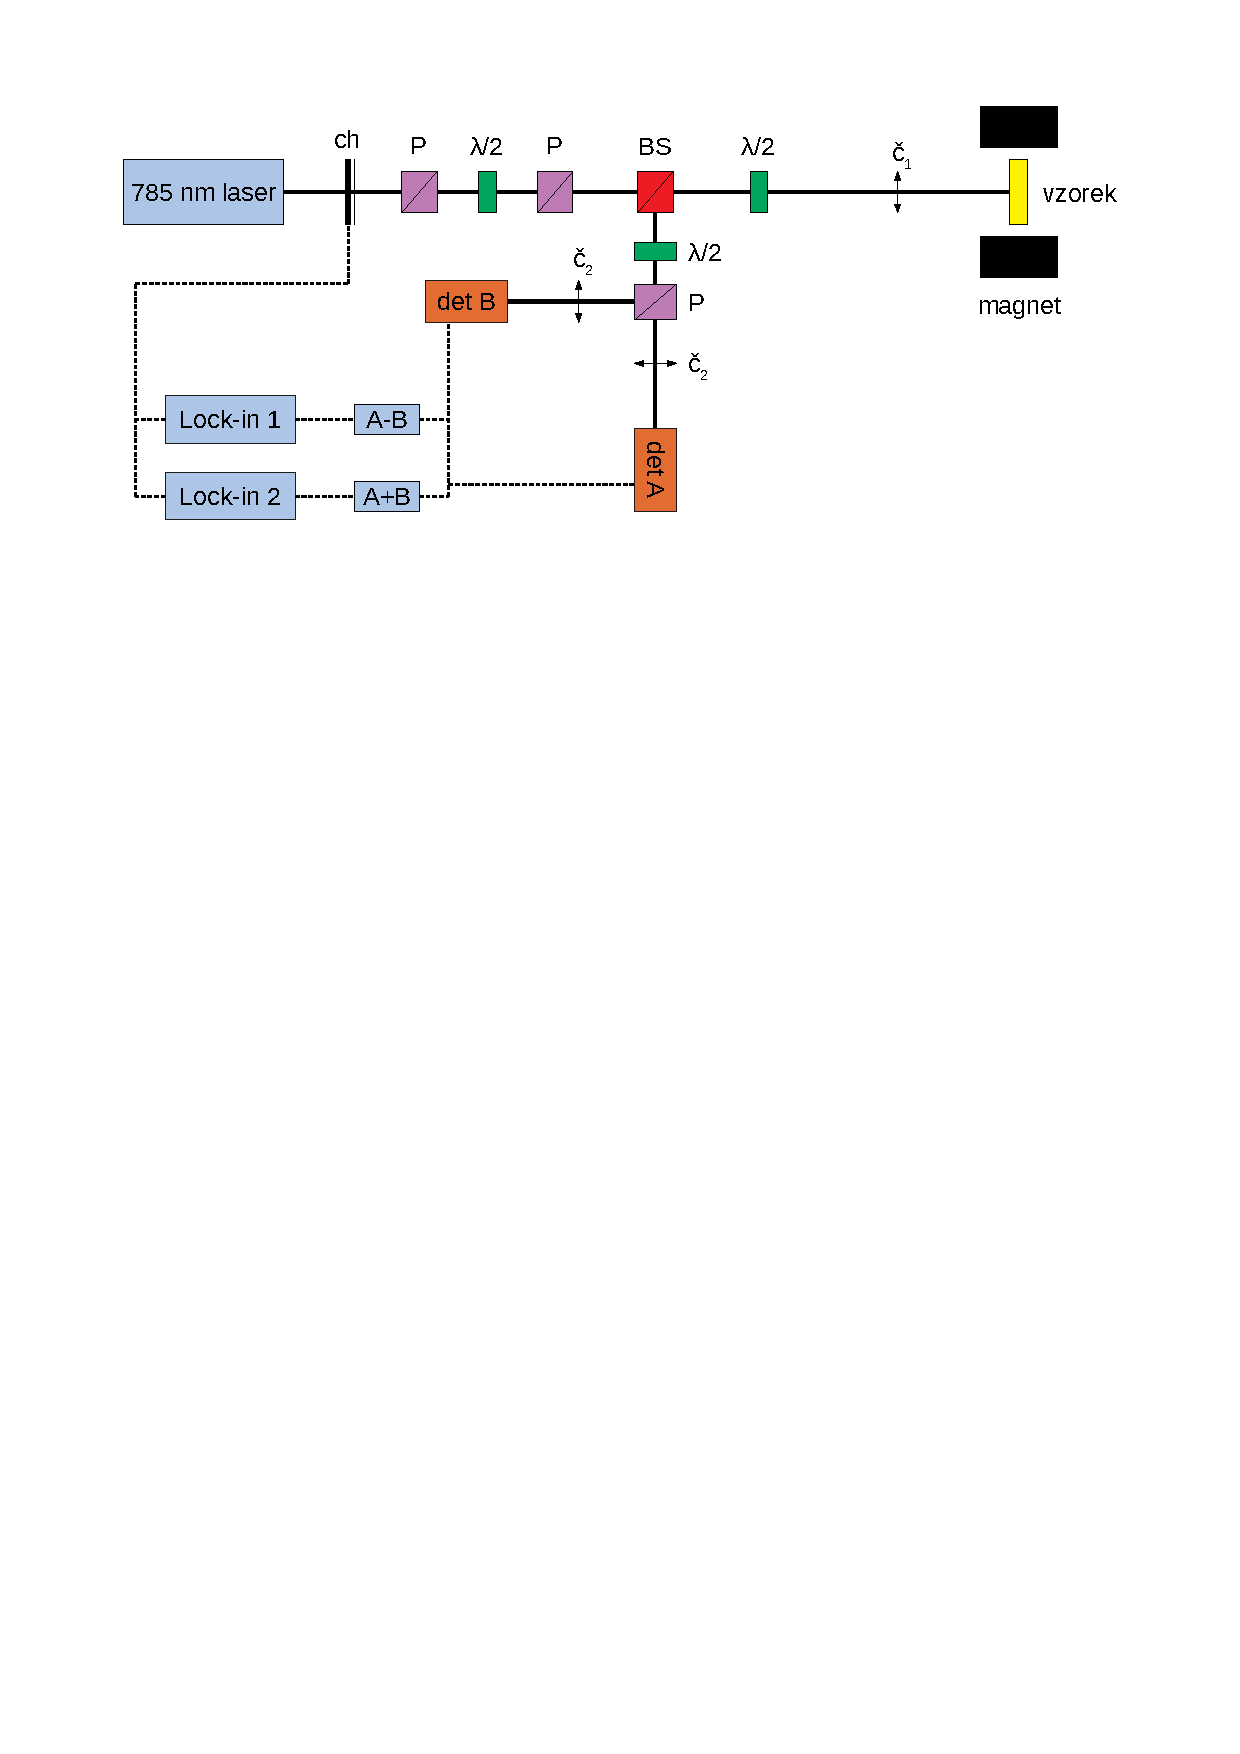
\includegraphics[trim={0,7in 8in 0,7in 0.5in}, clip, width=\textwidth]{./png/kolinearni_usporadani}
	\caption{Experimentální uspořádání v kolineární geometrii. ch --- přerušovač svazku, P --- polarizátor, $\lambda/2$ --- půlvlnná destička, č$_\text{i}$ --- spojná čočka, BS --- dělič svazku.}\label{kolinearni_usporadani}
\end{figure}

\FloatBarrier

\subsubsection*{Kryostat}

Protože GaMnAs má feromagnetické vlastnosti pouze za nízkých teplot, je do středu elektromagnetu zavedeno rameno kryostatu, který umožňuje nastavení teplot v rozmezí cca 5 až \SI{800}{\kelvin}. Vzorek je umístěn na tzv. studeném prstu (\emph{cold finger}) kryostatu. Kryostat je dále opatřen skleněnými okénky pro průchod světla. V~kryostatu jsou umístěny celkem tři teplotní čidla, křemíková dioda, platinové čidlo a termočlánek. Křemíková dioda je umístěná přibližně v půlce ramene kryostatu, zatímco platinové čidlo a termočlánek jsou blízko vzorku.
Při všech měřeních jsme zaznamenali teplotu všech čidel a určili skutečnou teplotu z dříve provedené kalibrace, viz obr. \ref{sensor}.

\begin{figure}[htbp]\centering
	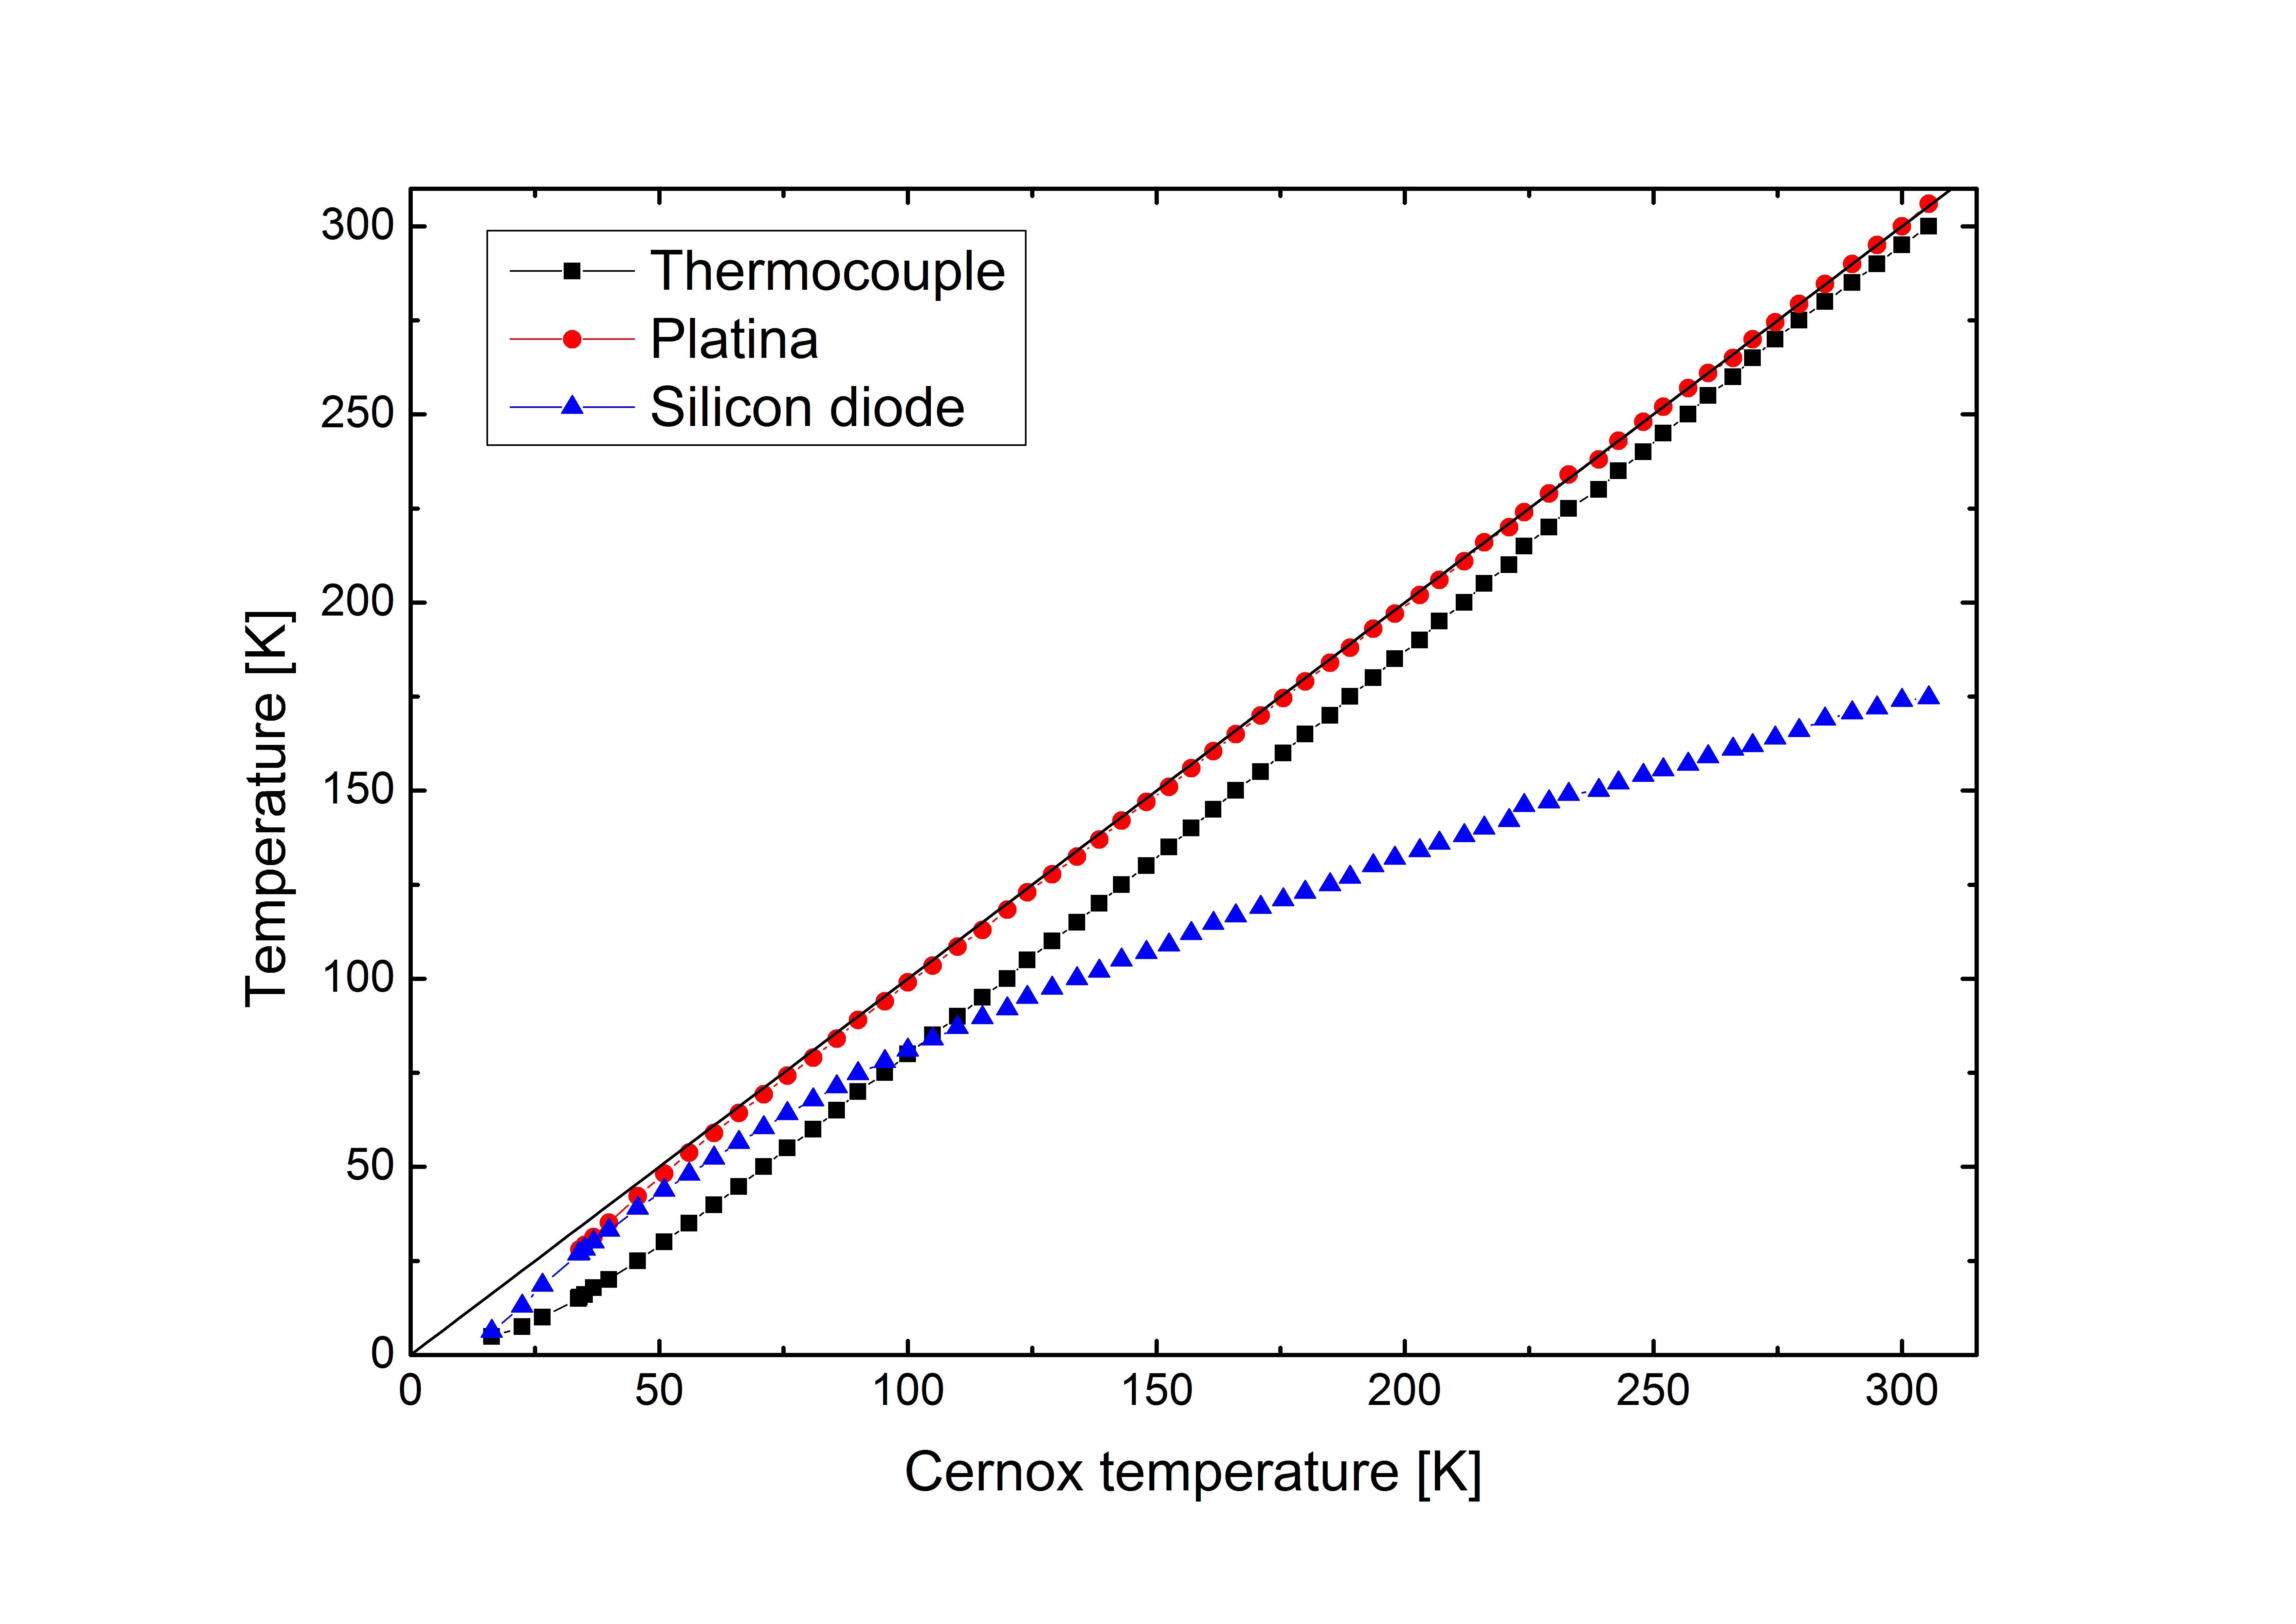
\includegraphics[width=0.8\textwidth]{./png/sensorcalibration}
	\caption{Kalibrace teplotních čidel. Na horizontální ose je skutečná teplota (měřená teplotním čidlem Cernox).}\label{sensor}
\end{figure}


Chladící výkon je vždy stejný a teplota se reguluje pouze topením. Při vypnutém topení dosáhne kryostat nejnižší možné teploty, kterou odhadujeme shora $T<\SI{15}{\kelvin}$. V grafech tato měření označujeme jako $T=\SI{12(3)}{\kelvin}$. Přestože procedura chlazení je vždy stejná, skutečná teplota se může při dvou zchlazeních lišit. Měření, u kterých uvádíme $T<\SI{15}{\kelvin}$, tedy neproběhla nutně při stejné teplotě. Každý typ měření (rozdělení do podkapitol) však proběhl ve stejný den při stejném zchlazení vzorku (bez změny nastavení termostatu).

Kryostat byl napojený na rotační a turbomolekulární vývěvu kvůli dosažení dostatečně nízkého tlaku (před zapnutím chlazení byl tlak \SI{2,5e-6}{\hecto\pascal}).